\chapter{\ifenglish Introduction\else บทนำ\fi}

\section{ที่มาและความสำคัญของปัญหา}

มะเร็งช่องปาก (Oral Cancer) ติดอันดับ 1 ใน 10 โรคที่พบบ่อยที่สุดในประเทศไทย
ความท้าทายสำคัญในชุมชนชนบทคือพฤติกรรมการซื้อยาปฏิชีวนะมารับประทานเองเมื่อมีแผลในช่องปาก
โดยไม่ปรึกษาแพทย์หรือทันตแพทย์ ส่งผลให้การวินิจฉัยล่าช้าและพบโรคในระยะลุกลาม
ทำให้ผลการรักษาแย่ลงอย่างมีนัยสำคัญ

%% >> แทนที่ด้วย: fig_bg_news.png
%% ที่มา: สไลด์ที่ 3 (ข่าว Amarin News)
\begin{figure}[H]
  \centering
  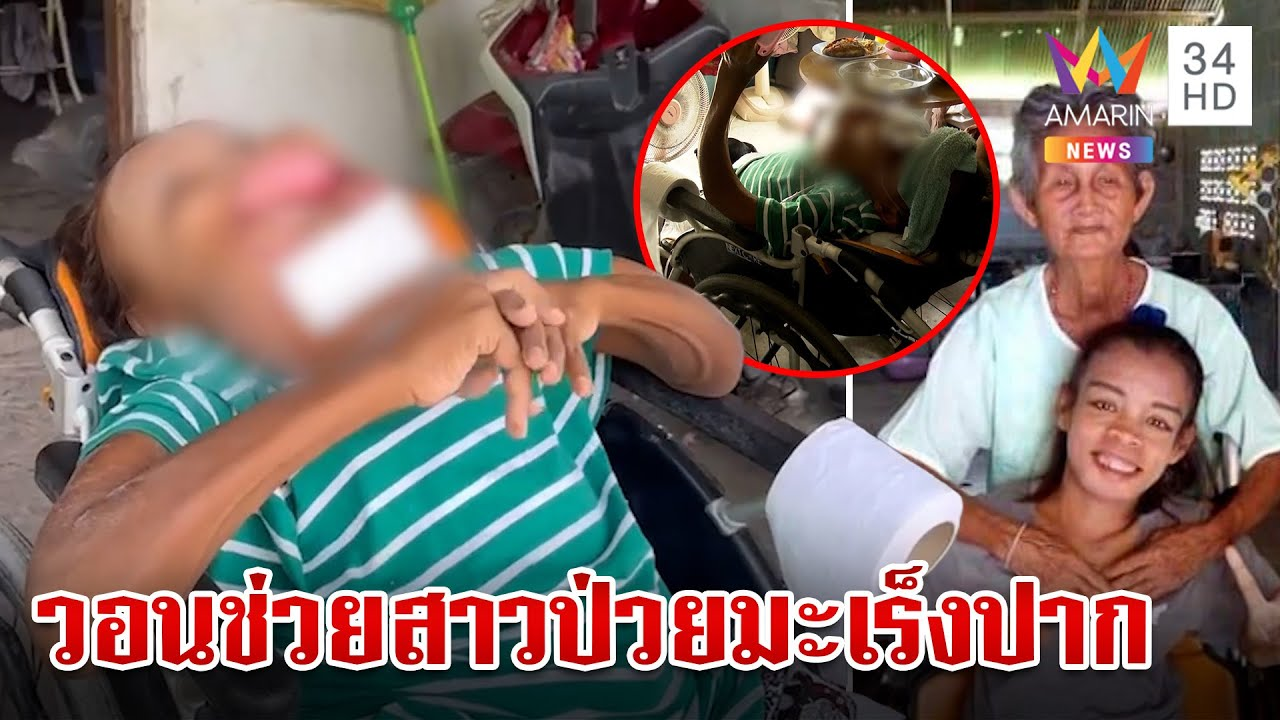
\includegraphics[width=0.9\linewidth]{fig/_bg/fig_bg_news.png}
  \caption{สื่อมวลชนรายงานปัญหาการวินิจฉัยมะเร็งช่องปากล่าช้า
    ผู้ป่วยในชนบทมักซื้อยามารับประทานเองจนอาการรุนแรง
    ที่มา: Amarin News / กรมอนามัย}
\end{figure}

ข้อมูลจากกรมอนามัย กระทรวงสาธารณสุข แบ่งรอยโรคในช่องปากออกเป็น 3 กลุ่มหลัก:

\begin{itemize}[leftmargin=1.8em, itemsep=3pt]
  \item \textbf{รอยโรคช่องปากทั่วไป (Oral Lesion)} --- พบมากที่สุด ครอบคลุมทุกช่วงอายุ
  \item \textbf{รอยโรคก่อนมะเร็ง (PMD --- Potentially Malignant Disorders)} ---
        รอยขาว (Leukoplakia) รอยแดง (Erythroplakia) ก้อน และแผลเล็กในช่องปาก
  \item \textbf{มะเร็งช่องปาก (OSCC --- Oral Squamous Cell Carcinoma)} ---
        พบมากในกลุ่มอายุ 60 ปีขึ้นไป
\end{itemize}

%% >> แทนที่ด้วย: fig_bg_lesion1.png และ fig_bg_lesion2.png
%% ที่มา: สไลด์ที่ 4
\begin{figure}[H]
  \centering
  \begin{minipage}[t]{0.48\linewidth}
    \centering
    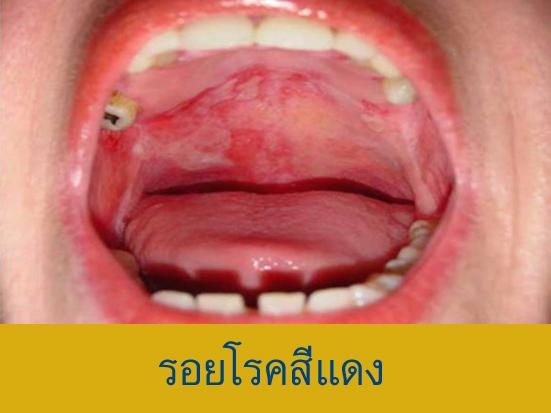
\includegraphics[width=\linewidth]{fig/_bg/fig_bg_lesion1.png}
    \caption{รอยโรคช่องปาก ตัวอย่างเคสที่ 1}
  \end{minipage}
  \hfill
  \begin{minipage}[t]{0.48\linewidth}
    \centering
    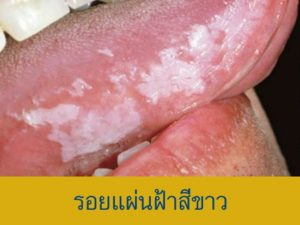
\includegraphics[width=\linewidth]{fig/_bg/fig_bg_lesion2.png}
    \caption{รอยโรคช่องปาก ตัวอย่างเคสที่ 2}
  \end{minipage}
\end{figure}

%% >> แทนที่ด้วย: fig_bg_lesion_annotated.png
%% ที่มา: สไลด์ที่ 5
\begin{figure}[H]
  \centering
  \begin{minipage}{0.65\linewidth}
    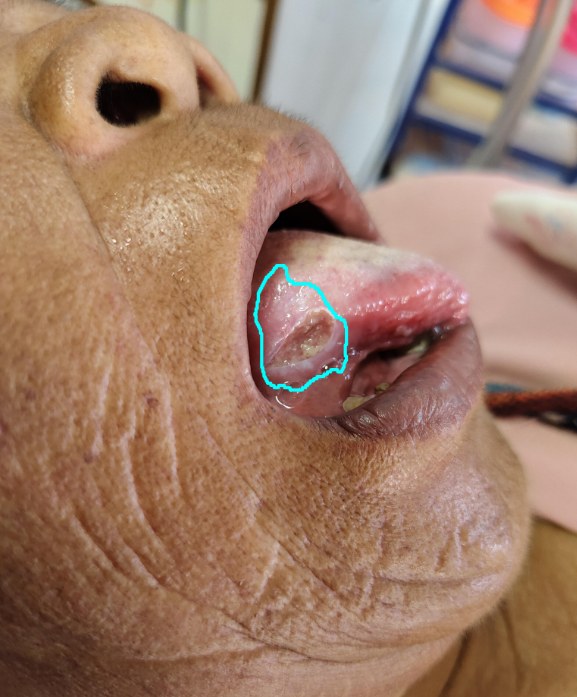
\includegraphics[width=\linewidth]{fig/_bg/fig_bg_lesion_annotated.png}
  \end{minipage}
  \caption{การ Annotation รอยโรคก่อนมะเร็งด้วย AI
    เส้นกรอบสีเหลืองแสดงบริเวณที่ส่งให้ผู้เชี่ยวชาญตรวจสอบ}
\end{figure}

%% >> แทนที่ด้วย: fig_bg_stats_chart.png
%% ที่มา: สไลด์ที่ 6
\begin{figure}[H]
  \centering
  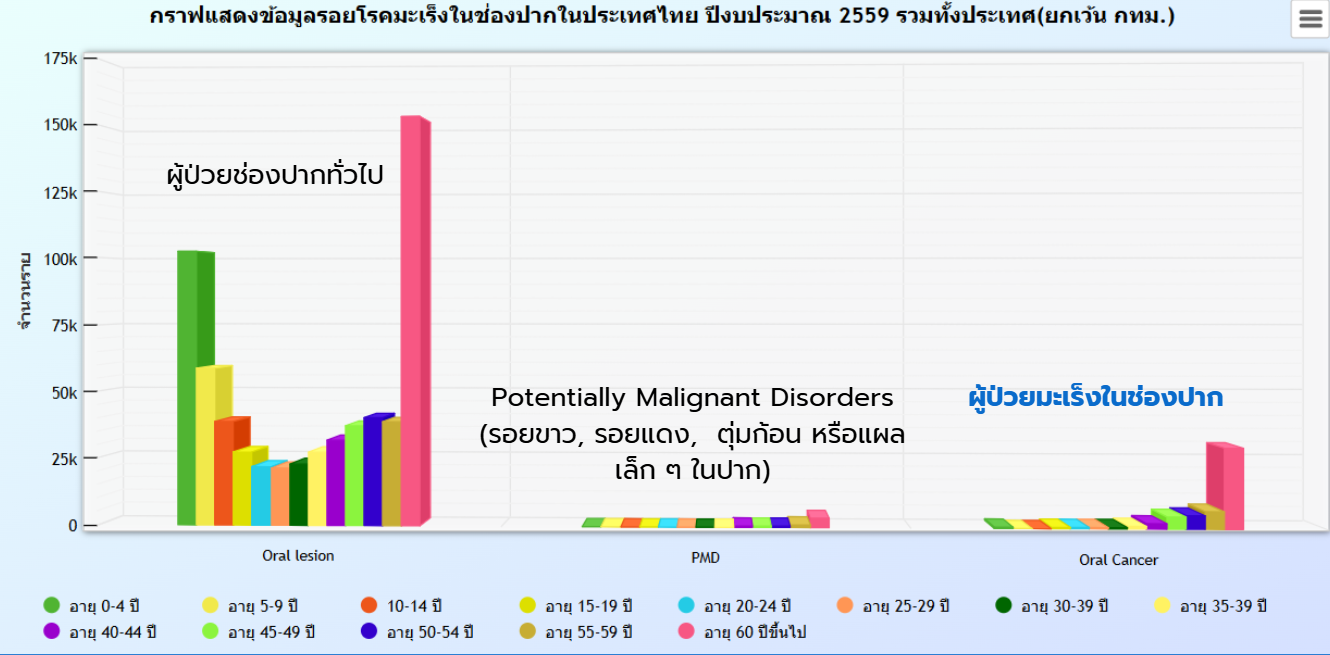
\includegraphics[width=0.95\linewidth]{fig/_bg/fig_bg_stats_chart.png}
  \caption{ข้อมูลรอยโรคช่องปากทั่วประเทศ ปีงบประมาณ 2559 (ยกเว้น กทม.)
    จำแนกเป็น 3 กลุ่ม ตามช่วงอายุ ที่มา: กรมอนามัย}
\end{figure}

%% >> แทนที่ด้วย: fig_bg_registry_table.png
%% ที่มา: สไลด์ที่ 7
\begin{figure}[H]
  \centering
  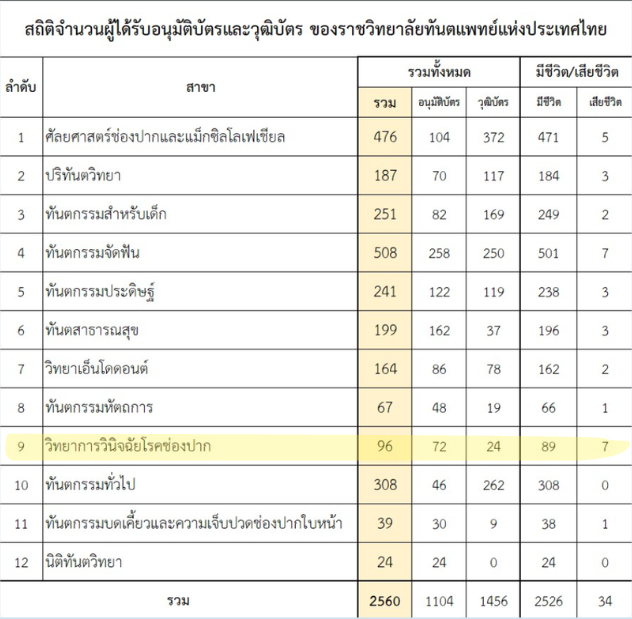
\includegraphics[width=0.95\linewidth]{fig/_bg/fig_bg_registry_table.png}
  \caption{จำนวนทันตแพทย์เฉพาะทาง ณ วันที่ 21 พฤศจิกายน 2567
    แถวที่ 9 (ไฮไลต์) สาขาวิทยาการวินิจัยโรคช่องปาก มีทันตแพทย์เพียง 96 คน}
\end{figure}

\begin{tcolorbox}[bluebox, title=ปัญหาหลัก]
  ผู้สูงอายุในชนบทอายุ 50 ปีขึ้นไป โดยเฉพาะกลุ่มเปราะบางที่พึ่งพาผู้ดูแล
  เผชิญอุปสรรคหนักในการเข้าถึงทันตแพทย์เฉพาะทาง
  เมื่อได้รับการวินิจฉัย มักพบว่าโรคลุกลามสู่ระยะท้ายแล้ว
  ส่งผลให้ผลการรักษาแย่ลงและค่าใช้จ่ายสูงขึ้นอย่างมาก
\end{tcolorbox}

\subsection{ข้อจำกัดทางเทคนิคของระบบเดิม}

แม้ระบบต้นแบบในเฟส~1 จะมีความแม่นยำของ AI ที่น่าพอใจ
แต่ยังไม่พร้อมสำหรับการใช้งานจริงในฐานะซอฟต์แวร์ทางการแพทย์
\textit{ในบริบทซอฟต์แวร์ทางการแพทย์ ความแม่นยำของ AI เพียงอย่างเดียวไม่เพียงพอ ---
ระบบต้องปลอดภัย โปร่งใส ตรวจสอบได้ และพร้อมใช้งานตลอดเวลา}
ระบบเดิมมีช่องโหว่สำคัญ 5 ประการ:

\begin{itemize}[leftmargin=1.8em, itemsep=4pt]
  \item \textbf{ไม่มีกรอบการปฏิบัติตาม PDPA / HIPAA} ---
        ข้อมูลสุขภาพผู้ป่วยถูกจัดเก็บโดยไม่ผ่านมาตรฐานคุ้มครองข้อมูลส่วนบุคคล
  \item \textbf{AI แบบ Monolith เป็น Single Point of Failure} ---
        หาก AI Service ล่ม ระบบทั้งหมดหยุดทำงานทันที ไม่มี Fallback
  \item \textbf{ไม่มีระบบ Audit Trail ป้องกันการแก้ไขย้อนหลัง} ---
        ไม่มีกลไกตรวจจับหรือป้องกันการแก้ไขเวชระเบียนย้อนหลัง
  \item \textbf{โค้ดแบบ Monolith ขยายระบบไม่ได้} ---
        การเปลี่ยนแปลงใดก็ตามเสี่ยงกระทบส่วนอื่น
        ไม่รองรับการ Scale Out แต่ละ Service
  \item \textbf{ไม่มี Role-Based Access Control (RBAC)} ---
        ผู้ใช้ทุกคนที่ผ่านการยืนยันตัวตนเข้าถึงข้อมูลและฟังก์ชันได้เหมือนกัน
\end{itemize}

\section{ระบบเดิม เฟส 1: AIDOC}

ระบบต้นแบบในเฟส~1 คือ \textbf{AIDOC}
(\textit{Artificial Intelligent System for Detecting and Analyzing PMDs and Oral Cancer})
พัฒนาและนำไปใช้งานร่วมกับกรมอนามัย
สร้างบน Flask Monolith Architecture ใช้ Bootstrap เป็น UI
จัดเก็บรูปภาพบน File System และใช้ MySQL เป็นฐานข้อมูล

%% >> แทนที่ด้วย: fig_aidoc_screenshot.png
%% ที่มา: สไลด์ที่ 8
\begin{figure}[H]
  \centering
  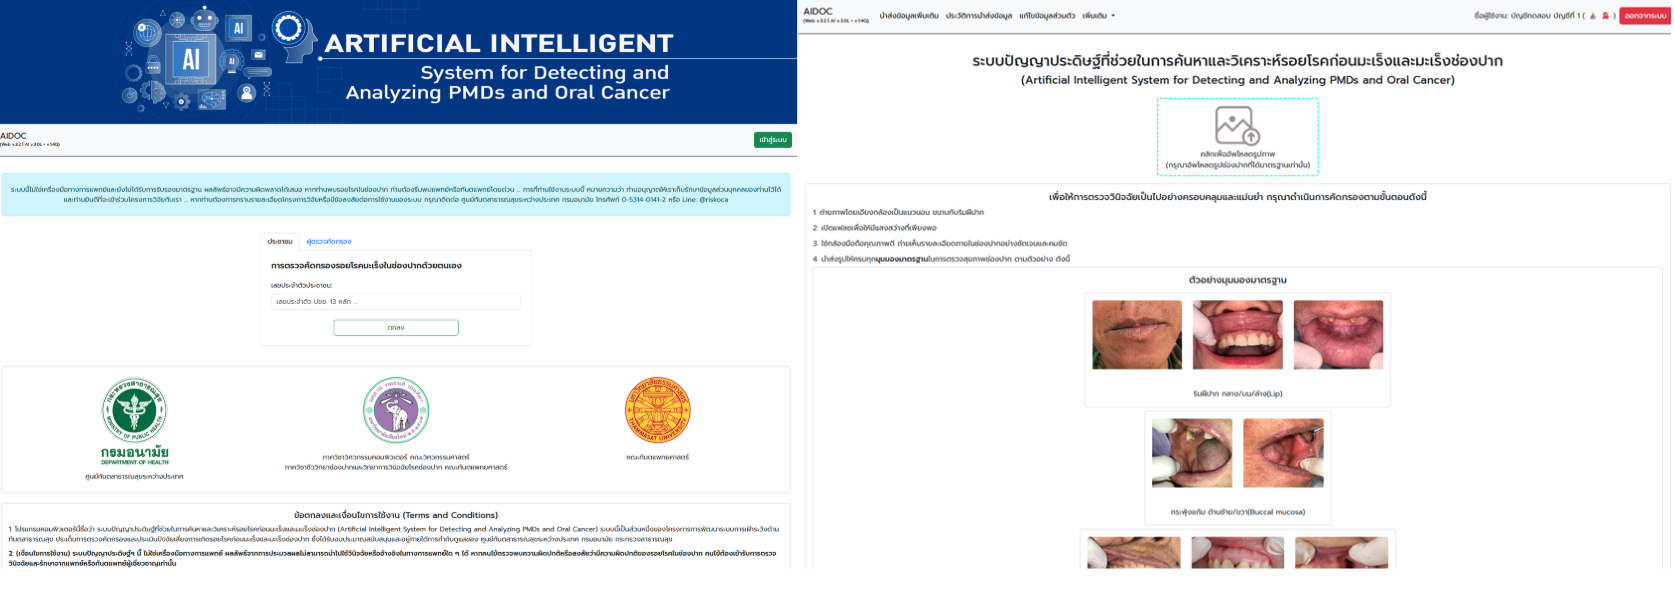
\includegraphics[width=0.95\linewidth]{fig/_bg/fig_aidoc_screenshot.png}
  \caption{ระบบ AIDOC เฟส 1: (ซ้าย) หน้า Consent และ Login;
    (ขวา) Workflow อัปโหลดภาพและคัดกรองด้วย AI
    สร้างด้วย Flask + Bootstrap + MySQL}
\end{figure}

\section{ข้อจำกัดของระบบเฟส 1}

\begin{tcolorbox}[bluebox]
  \centering\itshape
  ``ซอฟต์แวร์ทางการแพทย์ต้องมีความปลอดภัย โปร่งใส ตรวจสอบได้ และพร้อมใช้งานตลอดเวลา''
\end{tcolorbox}

%% >> แทนที่ด้วย: fig_legacy_arch.png
%% ที่มา: สไลด์ที่ 9 / 18
\begin{figure}[H]
  \centering
  \begin{minipage}{0.72\linewidth}
    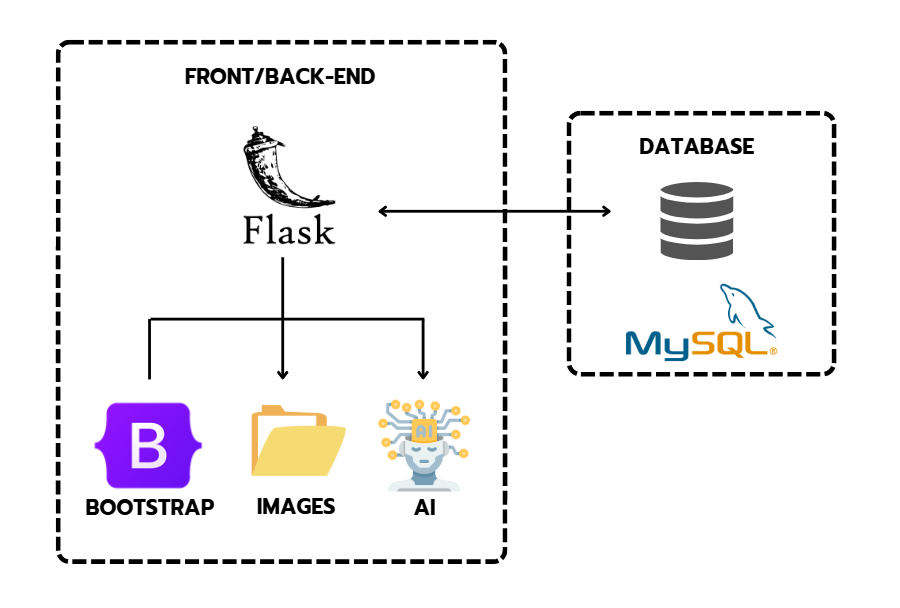
\includegraphics[width=\linewidth]{fig/_bg/fig_legacy_arch.png}
  \end{minipage}
  \caption{สถาปัตยกรรมระบบเดิม: Flask ทำหน้าที่ทั้ง Frontend, Backend, AI Inference
    และ Image Storage ในหน่วยเดียว ความล้มเหลวของส่วนใดทำให้ระบบทั้งหมดหยุด}
\end{figure}

\vspace{4pt}
\renewcommand{\arraystretch}{1.4}
\begin{tabularx}{\linewidth}{|>{\bfseries\color{primaryblue}}p{0.32\linewidth}|X|}
  \hline
  \rowcolor{primaryblue}
  \textcolor{white}{\textbf{ข้อจำกัด}} & \textcolor{white}{\textbf{ผลกระทบ}}\\
  \hline
  ไม่มีการปฏิบัติตาม PDPA / HIPAA &
    ข้อมูลผู้ป่วยขาดการคุ้มครองตามกฎหมายและข้อกำหนดที่เกี่ยวข้อง\\
  \hline
  Single Point of Failure &
    หาก Flask ล่ม ระบบทั้งหมดใช้งานไม่ได้ทันที\\
  \hline
  ไม่มี Audit Trail ป้องกันการแก้ไขย้อนหลัง &
    เวชระเบียนสามารถถูกแก้ไขโดยไม่มีหลักฐาน\\
  \hline
  โค้ดแบบ Monolith ขยายระบบยาก &
    การแก้ไข Bug หรืออัปเดต AI เสี่ยงทำให้ระบบอื่นพัง\\
  \hline
\end{tabularx}

\section{วิธีดำเนินงาน: การ Re-engineer สถาปัตยกรรมระบบ}

วิธีดำเนินงานหลักของเฟส~2 คือการ Re-engineer สถาปัตยกรรมระบบใหม่ทั้งหมด
โดยแบ่งออกเป็น 4 เสาหลักทางวิศวกรรม:

\subsection{เสาหลักที่ 1: Architecture Re-engineering}

\begin{itemize}[leftmargin=1.8em, itemsep=3pt]
  \item \textbf{Next.js} (Layered Design, Mobile-first) สำหรับ Frontend
        พร้อม Auth Guard และการแยก State Management
  \item \textbf{FastAPI + Clean Architecture + Domain-Driven Design (DDD)}
        สำหรับ Backend --- Business Logic แยกจาก AI Layer อย่างสมบูรณ์
  \item \textbf{Async Queue Processing} (Redis + Celery Workers)
        ขจัดปัญหาเว็บค้างและ API Timeout จาก Synchronous AI Inference
\end{itemize}

\subsection{เสาหลักที่ 2: High-Availability AI (Dual-Path Inference)}

\begin{itemize}[leftmargin=1.8em, itemsep=3pt]
  \item \textbf{Primary Path:} NVIDIA Triton Inference Server (GPU, gRPC)
        พร้อม TensorRT Optimization
  \item \textbf{Fallback Path:} TensorFlow Lite (CPU, HTTP)
        พร้อม Auto Failover อัตโนมัติ
  \item \textbf{Health Monitoring:} ตรวจสอบสถานะต่อเนื่อง
      เปิด Auto-Switch ภายในเวลาไม่เกิน $\leq 1\,\text{s}$
\end{itemize}

\subsection{เสาหลักที่ 3: Data and Processing Layer}

\begin{itemize}[leftmargin=1.8em, itemsep=3pt]
  \item \textbf{PostgreSQL} (OLTP + Audit) --- ฐานข้อมูลหลักพร้อม Immutable Audit Schema
  \item \textbf{Redis} --- Task Queue สำหรับงาน AI แบบ Async และ Cache
  \item \textbf{MinIO} --- Object Storage สำหรับรูปภาพทางคลินิก
  \item \textbf{Celery Workers} --- ประมวลผลเบื้องหลัง: AI Inference Queue,
        2-Tier Audit Chain, Archival และงาน Compliance
\end{itemize}

\subsection{เสาหลักที่ 4: Enterprise Security and Compliance}

\begin{itemize}[leftmargin=1.8em, itemsep=3pt]
  \item \textbf{TLS 1.3} เข้ารหัสการสื่อสารทุกส่วนแบบ End-to-End
  \item \textbf{Role-Based Access Control (RBAC)} ครอบคลุม 6 บทบาท:
        ผู้ป่วย, อสม., ทันตแพทย์, ผู้คัดกรอง, ผู้เชี่ยวชาญ, ผู้ดูแลระบบ
  \item \textbf{2-Tier Audit Logging + Hash-Chain} ป้องกันการแก้ไขย้อนหลัง
        ตรวจสอบได้ 100\%
  \item \textbf{PDPA / HIPAA-ready} สอดคล้องกับกฎหมายคุ้มครองข้อมูลส่วนบุคคลของไทย
\end{itemize}

\section{แนะนำ eDENT-ELDER เฟส 2}

\subsection{วิสัยทัศน์และคำขวัญ}

\begin{tcolorbox}[bluebox]
  \centering
  {\large\bfseries ``พบเร็ว \textendash{} ส่งต่อเร็ว \textendash{} ติดตามครบ''}\\[0.4em]
  \textit{``Detect Early \textemdash{} Refer Fast \textemdash{} Follow Up Completely''}
\end{tcolorbox}

\subsection{กลุ่มเป้าหมาย}

\begin{enumerate}[leftmargin=1.8em, label=\textbf{\arabic*.}, itemsep=4pt]
  \item \textbf{ผู้สูงอายุที่มีอายุ 50 ปีขึ้นไป} ---
        กลุ่มเปราะบาง อาศัยในชนบท และต้องพึ่งพาผู้ดูแล
  \item \textbf{บุคลากรสาธารณสุขแนวหน้า} ---
        อาสาสมัครสาธารณสุขประจำหมู่บ้าน (อสม.) ทันตาภิบาล
        และเจ้าหน้าที่ รพ.สต. ที่ผ่าน Train-the-Trainer 6--8 รุ่น
\end{enumerate}

\subsection{4 เสาหลักของแพลตฟอร์ม}

\begin{tcolorbox}[graybox]
  \renewcommand{\arraystretch}{1.5}
  \begin{tabularx}{\linewidth}{@{}>{\bfseries\color{primaryblue}}p{0.26\linewidth}X@{}}
    Hybrid Mobile Platform &
      อินเทอร์เฟซที่ใช้งานง่ายผ่านมุมมองมือถือ และ Web Dashboard
      สำหรับผู้ดูแลและเจ้าหน้าที่ภาคสนาม\\
    AI-Guided Screening &
      AI ตรวจจับรอยโรค OPMD/OSCC พร้อม Assisted-Capture
      และ Quality-Gate รับรองคุณภาพภาพถ่าย\\
    Elderly-Centric Empowerment &
      เสริมพลัง อสม. (อายุ 50+) ในการคัดกรอง
      สื่อสารความเสี่ยง และส่งต่ออย่างเป็นระบบ\\
    Asynchronous Teleconsultation &
      ระบบ Store-and-Forward เชื่อมต่อ อสม. กับผู้เชี่ยวชาญ
      โดยไม่ต้องนัดหมายพร้อมกัน\\
  \end{tabularx}
\end{tcolorbox}

\section{วัตถุประสงค์ของโครงงาน}

\begin{enumerate}[leftmargin=1.8em, label=\textbf{\arabic*.}, itemsep=6pt]
  \item \textbf{พัฒนาและทดสอบระบบ AI คัดกรอง} OPMD/OSCC ให้มีความแม่นยำสูง
    ใช้งานได้จริงในภาคสนาม และได้รับการยอมรับจากทันตแพทย์เฉพาะทาง
  \item \textbf{พัฒนาแพลตฟอร์ม eDENT-ELDER} รองรับการคัดกรองด้วยตัวเองและการคัดกรองชุมชน
  \item \textbf{ประเมินผลลัพธ์ด้านบริการและสังคม} วัดการเข้าถึง เวลาพบผู้เชี่ยวชาญ
        อัตราตรวจพบระยะแรก และความยั่งยืน
\end{enumerate}

\subsection{ประโยชน์ที่คาดว่าจะได้รับ}

\begin{itemize}[leftmargin=1.8em, itemsep=4pt]
  \item \textbf{ระดับระบบ:} แพลตฟอร์มที่ผสาน AI ปลอดภัย ตรวจสอบได้
        ลดภาระแนวหน้าและเพิ่มโอกาสตรวจพบระยะแรก (Stage-Shift)
  \item \textbf{ระดับชุมชน:} ผู้สูงอายุและครอบครัวในพื้นที่นำร่องได้รับการคัดกรองเร็วขึ้น
        หัวหน้า อสม. (อายุเฉลี่ย 50+) เป็นทั้งผู้ให้บริการและผู้รับประโยชน์
\end{itemize}

\begin{tcolorbox}[graybox]
  \textbf{พื้นที่นำร่องหลัก:}
  เชียงใหม่ \textbullet{} พะเยา \textbullet{} ภูเก็ต \textbullet{} หนองบัวลำภู\\
  \textbf{เครือข่ายเสริม:} สุรินทร์ สมุทรปราการ และจังหวัดอื่นตามความพร้อม
\end{tcolorbox}

\section{ภาคีและผู้ร่วมดำเนินงาน}

\renewcommand{\arraystretch}{1.3}
\begin{tabularx}{\linewidth}{lX}
  \toprule
  \textbf{หน่วยงาน} & \textbf{บทบาท}\\
  \midrule
  คณะทันตแพทยศาสตร์ มหาวิทยาลัยธรรมศาสตร์ &
    คำปรึกษาทางคลินิกและเครือข่ายผู้เชี่ยวชาญ\\
  คณะวิศวกรรมศาสตร์ มหาวิทยาลัยเชียงใหม่ &
    ทีมพัฒนาระบบ\\
  คณะทันตแพทยศาสตร์ มหาวิทยาลัยเชียงใหม่ &
    ตรวจสอบและให้ Feedback ทางคลินิก\\
  กรมอนามัย ศูนย์ทันตสาธารณสุขระหว่างประเทศ เชียงใหม่ &
    ความร่วมมือด้านข้อมูลและการ Deploy\\
  NurseCMU &
    บูรณาการงานสาธารณสุขชุมชน\\
  \bottomrule
\end{tabularx}

